\documentclass{beamer}

\usepackage[utf8]{inputenc}
\usepackage{default}
\usepackage{pslatex}
\usepackage{graphicx}
\usepackage{algorithmic}
\usepackage{multicol}

\usetheme{Warsaw}

\title{Comment simuler numériquement la géomorphologie alpine ?}
\subtitle{Sujet de TPE}
\author{Gros Alexis, Manceau Thibaut, Porteries Tristan}
% \logo{
\includegraphics[height=0.5cm]{blender.png}}

\makeindex

\useoutertheme{infolines}

\begin{document}

% Titre
\frame{\titlepage}

% Sommaire
\begin{frame}{Sommaire}
\small \tableofcontents
\end{frame}

\section{Les phénomènes géormophologiques}
\subsection{La subduction}
\begin{frame}
\end{frame}

\subsection{L'obduction}
\begin{frame}
\end{frame}

\section{L'érosion}
\subsection{L'altération mécanique}
\begin{frame}
\end{frame}

\subsection{L'altération physico-chimique}
\begin{frame}
\end{frame}

\section{Le système cellulaire}
\subsection{Les cellules}
\begin{frame}
\end{frame}

\section{Les interactions entre cellules}
\subsection{Loi du centre instantané de rotation}
\begin{frame}
  $\overleftarrow{u}$ = vitesse verticale
  $\overleftarrow{v}$ = vitesse horizontale
  $\alpha$ = $\beta$ = la rotation en radians par secondes
  $\overleftarrow{u}$ = vitesse de 
  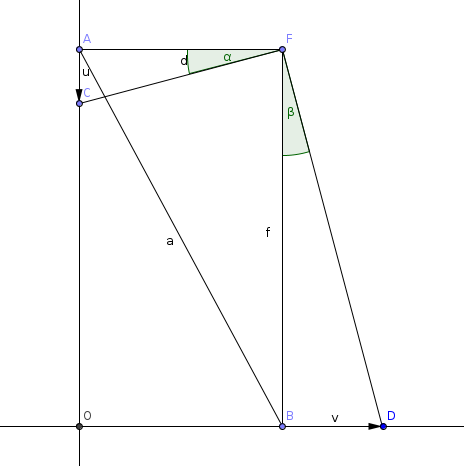
\includegraphics[width=5cm]{geogebra_1.png}
\end{frame}

\begin{frame}
  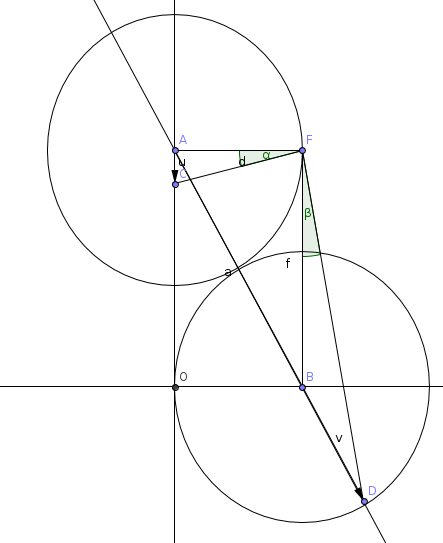
\includegraphics[width=6cm]{geogebra_2.png}
\end{frame}


\subsection{La loi de Hook et le module de Young}
\begin{frame}
\end{frame}

\subsection{La loi de Coulomb}
\begin{frame}
\end{frame}

\section{Les images de simulation}
\begin{frame}
\end{frame}






\end{document}
